\documentclass[10pt]{beamer}

\usetheme{Frankfurt}
\useoutertheme{default}
\setbeamertemplate{footline}[page number]
\setbeamertemplate{navigation symbols}{}

\usepackage{cmap}					% поиск в PDF
\usepackage[T2A]{fontenc}			% кодировка
\usepackage[utf8]{inputenc}			% кодировка исходного текста
\usepackage[english,russian]{babel}	% локализация и переносы
\usepackage{indentfirst}
\usepackage{subfig}
\usepackage{graphicx}
\usepackage{caption}
\usepackage{booktabs}
\frenchspacing

\newcommand{\bz}{\ensuremath{\boldsymbol{z}}}
\newcommand{\bx}{\ensuremath{\boldsymbol{x}}}
\newcommand{\bbx}{\ensuremath\bar{{\boldsymbol{x}}}}
\newcommand{\tbx}{\ensuremath{\tilde{\boldsymbol{x}}}}
\newcommand{\tbz}{\ensuremath{\tilde{\boldsymbol{z}}}}
\newcommand{\beps}{\ensuremath{\boldsymbol{\epsilon}}}
\newcommand{\delayV}[1]{\overset{\leftarrow}{\boldsymbol{x}}({#1})}

\title{Классификация временных рядов \\ динамических систем}
\author{Кирилл Сёмкин}
\institute[MIPT]{Московский физико-технический институт \\ Кафедра интеллектуальных систем}
\date[2026]{\textit{Научный руководитель}: д.ф.-м.н. В.\,В.~Стрижов \\ 2026}

\begin{document}

	\begin{frame}[c]
		\titlepage
	\end{frame}

	\begin{frame}{Задача классификации временных рядов}

		\begin{itemize}
			\item \emph{Многомерный временной ряд} --- последовательность случайных векторов произвольной длины $n$ $\bx(t_i) = \{\bx_{t_1}, \ldots, \bx_{t_n}\}$, $\bx_{t_i} \in \mathbb{R}^d$, в моменты $t_1, \ldots, t_n$.
			\item Каждому ряду соответствует метка класса (случайная величина) $y \in 1 \ldots K$.
			\item \emph{Классификатор} --- отображение $\delta\big(\bx(t_i)\big)$, относящее ряд к классу.
		\end{itemize}

		\begin{figure}[h]
			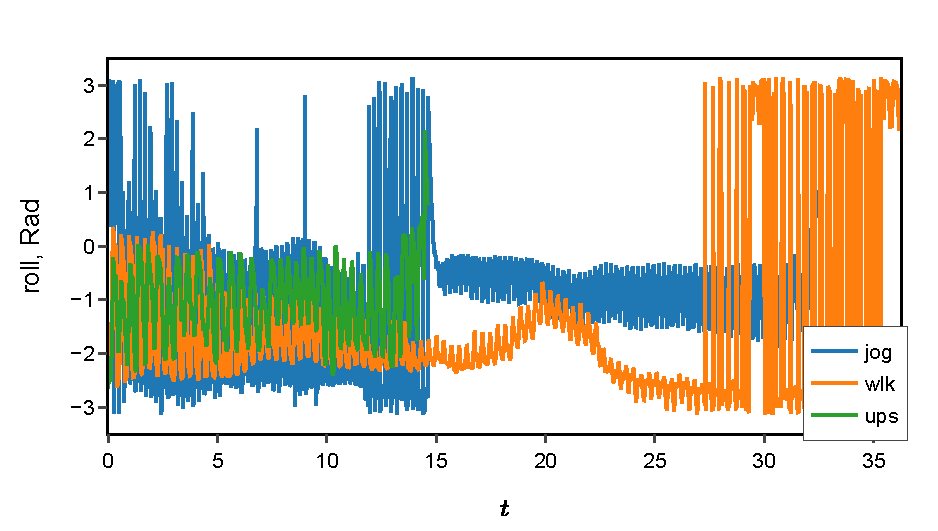
\includegraphics[width=0.7\textwidth, keepaspectratio]{img/time_series_viz}
			\caption*{Временные ряды трёх разных классов (IMU-сенсор)}
		\end{figure}

	\end{frame}

	\begin{frame}{Модель временных рядов --- динамическая система}

		Классу $j$ соответствует векторное поле $f_j \in \mathcal{F}(M)$. Ряд --- зашумлённая фазовая траектория ОДУ
		\begin{equation}\label{eq:lat_dyn}
			\begin{cases}
				\frac{d}{dt} \bbx(t) = f_j(\bbx), \\
				\bbx(0) = \bbx_0,
			\end{cases}
			\qquad
			\bx(t_i) = \bbx(t_i) + \beps(t_i),
		\end{equation}
		где шум $\beps_{t_i}$ --- i.i.d. случайные векторы:
		\begin{equation*}
			\mathbb{E}[\beps_{t_i}] = 0, \quad \text{Cov}(\beps_{t_i}) = R, \quad \lVert R \rVert_2 \le \sigma^2 < \infty.
		\end{equation*}

		\vspace{0.3em}
		Более общая модель --- СДУ, фазовая траектория которой случайна:
		\begin{equation}\label{eq:sde_dyn}
			\begin{cases}
				d\bbx(t) = f_j(\bbx)dt + G_j \, dW(t), \\
				\bbx(0) = \bbx_0,
			\end{cases}
		\end{equation}
		где $W(t)$ --- $m$-мерное броуновское движение, $G_j$ --- матрица диффузии класса.

		\vspace{0.3em}
		Решение задачи Коши (IVP) обозначаем $\bbx(t \,|\, \bbx_0, f_j)$.

	\end{frame}

	\begin{frame}{Восстановление фазовых траекторий по временным рядам}

		Пусть наблюдается не сама траектория, а её образ $\bx(t_i) = \alpha(\bbx(t_i)) + \beps(t_i)$, где $\alpha: M \to \mathbb{R}^d$, $\dim M = k$. Восстановление $\bbx(t_i)$ --- через диффеоморфизм многообразий:

		\begin{itemize}
			\item \textbf{Теорема Уитни}: наблюдается $2k+1$ рядов и $\alpha$ --- типичное вложени $\Rightarrow$ наблюдения уже являются диффеоморфной траекторией
			\item \textbf{Теорема Такенса}: достаточно \emph{одного} скалярного ряда --- вложение строится из векторов задержек $\big( x(t_i), x(t_{i-1}), \ldots, x(t_{i-m})\big)$, $m > 2k$.
		\end{itemize}

		\begin{figure}[h]
			\centering
			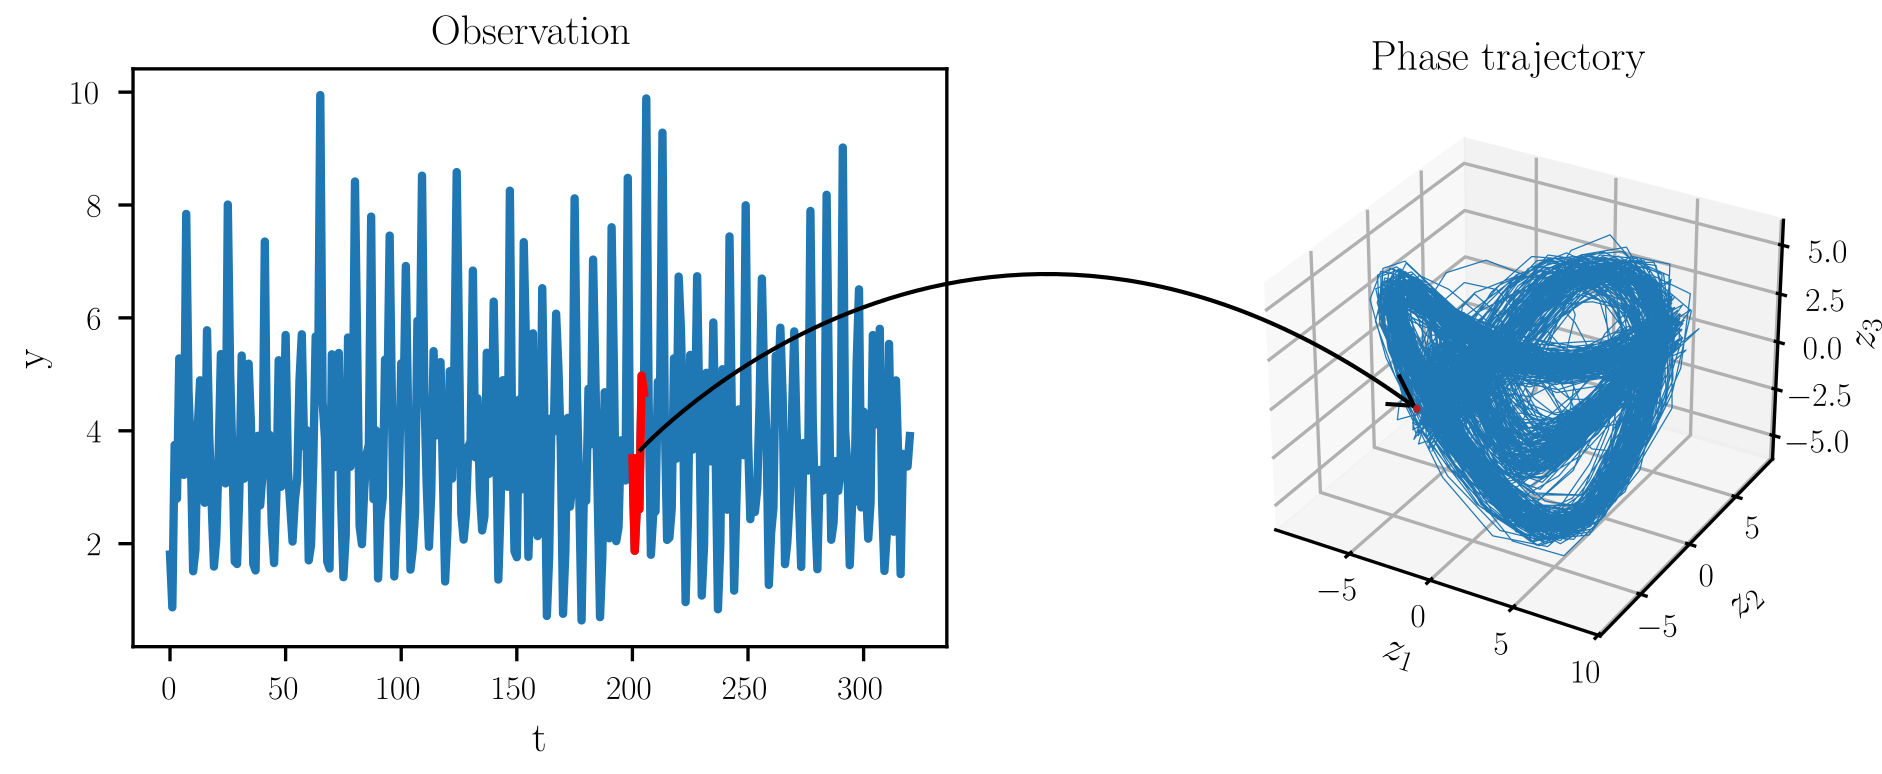
\includegraphics[width=0.52\textwidth, keepaspectratio]{img/takens}
			\caption*{\footnotesize Точка траектории $\bbx(t_i)$ собирается из лаговых значений ряда. Далее не различаем восстановленные и исходные траектории.}
		\end{figure}

	\end{frame}

	\begin{frame}{Метрический классификатор и его асимптотическая оптимальность}

		Введём метрику $\rho_n\big( \bx(t_i), \bz(t_i) \big) = \sum_{i=1}^n \lVert \bx_{t_i} - \bz_{t_i} \rVert_2^2$ и определим классификатор
		\begin{equation*}
			\delta \big( \bx(t_i) \big) = \underset{j \in 1 \ldots K}{\arg\min} \ \rho_n\big( \bx(t_i), \bbx(t_i \,|\, \bbx_0, f_j) \big).
		\end{equation*}

		\begin{block}{Теорема (Сёмкин, 2026)}
			Пусть $\bbx_0$ известна точно, шум удовлетворяет условиям модели и траектории классов расходятся:
			\begin{equation*}
				\rho_{\infty} \big( \bbx(t_i | \bbx_0, f_j), \bbx(t_i | \bbx_0, f_p) \big) = +\infty \quad \forall j \not= p.
			\end{equation*}
			Тогда вероятность ошибки классификации стремится к нулю:
			\begin{equation*}
				\mathbb{P}\big(\delta ( \bx(t_i) ) \not= y\big) \to 0, \quad n \to \infty.
			\end{equation*}
		\end{block}

		\footnotesize Доказательство --- через неравенство Чебышёва и union bound; порядок сходимости $\mathcal{O}\big( \sigma^2 / \rho_n \big)$.

	\end{frame}

	\begin{frame}{Погрешности поля и ОДУ-солвера могут ухудшать качество классификации}

		\begin{columns}[T]
			\begin{column}{0.48\textwidth}
				\centering
				$\lVert f - \tilde{f} \rVert \le 0.1$, но траектории расходятся: центр против устойчивого фокуса

				\vspace{0.3em}
				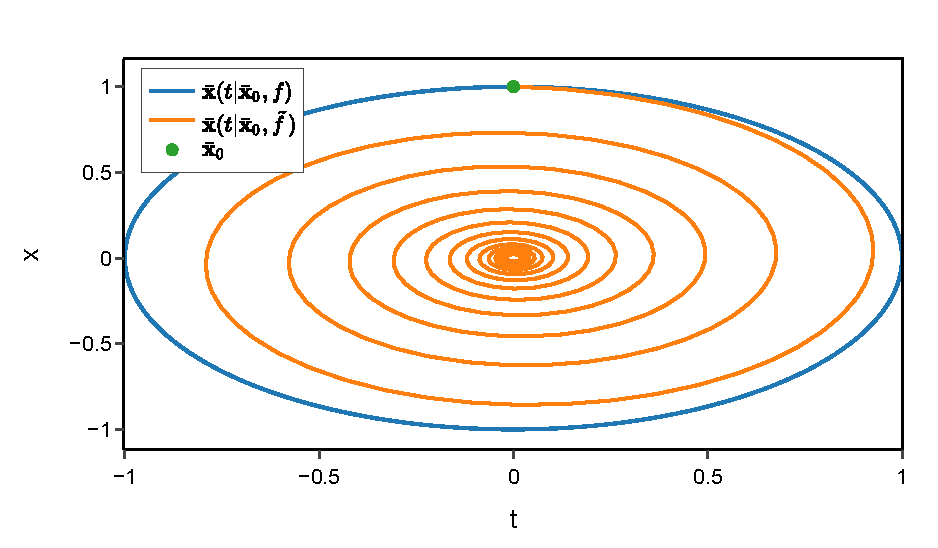
\includegraphics[width=\linewidth, keepaspectratio]{img/diverging_systems}
			\end{column}
			\begin{column}{0.48\textwidth}
				\centering
				Жёсткая система: метод Эйлера с шагом $\tau=0.05$ неустойчив, RK23 --- точен

				\vspace{0.3em}
				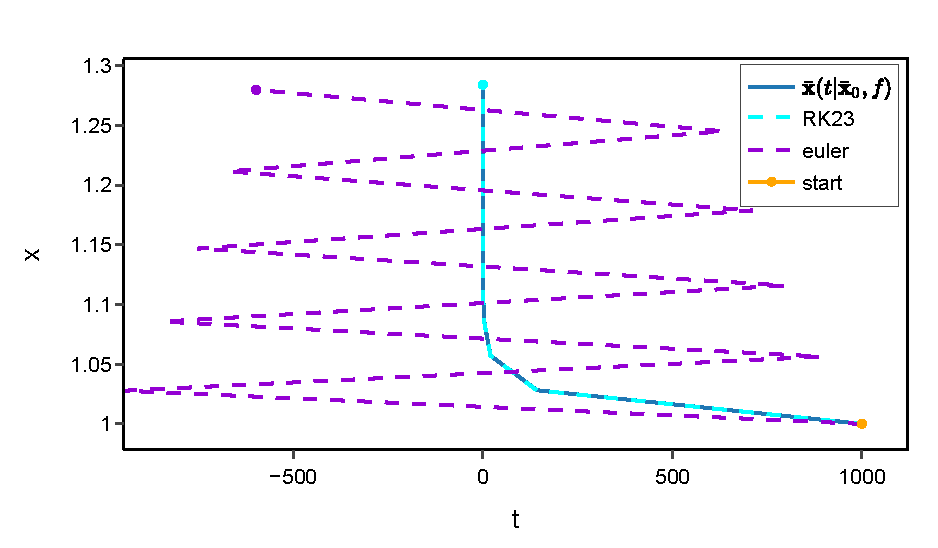
\includegraphics[width=\linewidth, keepaspectratio]{img/stiffness_illustration}
			\end{column}
		\end{columns}

		\vspace{0.8em}
		Кроме того, начальная точка случайна, $\bbx_0 \sim F(\cdot)$ $\Rightarrow$ точное IVP $\bbx(t_i \,|\, \bbx_0, f_j)$ в классификаторе недостижимо на практике.

	\end{frame}

	\begin{frame}{Сглаживание: условное матожидание вместо точного решения}

		\begin{columns}[T]
			\begin{column}{0.5\textwidth}
				Разобьём динамику на отрезки $[t_i, t_{i+1})$ и аппроксимируем $\bbx(t_i \,|\, \bbx_0, f_j)$ солвером:
				\begin{equation}\label{eq:state_space_ode}
					\small
					\begin{cases}
						\bbx_{t_{i+1}} = \text{ODESolve}(t_{i+1} - t_i \,|\, \bbx_{t_i}, f), \\
						\bx_{t_i} = \bbx_{t_i} + \beps_{t_i}, \\
						\bbx_0 \sim F(\cdot).
					\end{cases}
				\end{equation}
			\end{column}
			\begin{column}{0.46\textwidth}
				\centering
				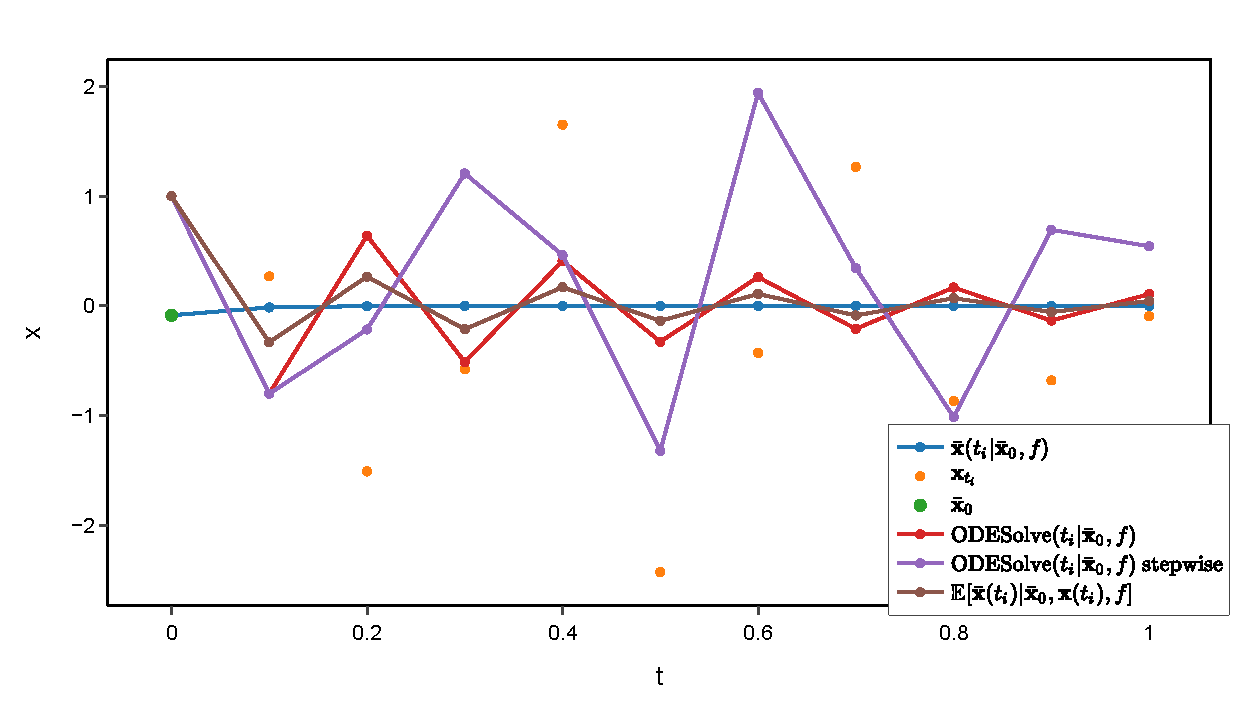
\includegraphics[width=\linewidth, keepaspectratio]{img/ode_cls_compare}

				{\footnotesize ОДУ $f(x) = -18x$: UKF точнее солверов с вероятностью $0.92$ по оценке Монте-Карло}
			\end{column}
		\end{columns}

		\vspace{0.7em}
		Наилучшее $L_2$-приближение IVP по имеющимся данным --- условное матожидание $\mathbb{E}[\bbx(t_i) \,|\, \bbx_0, \bx(t_i), f]$. Его нахождение в условиях (\ref{eq:state_space_ode}) --- \emph{задача сглаживания}. Новый классификатор:
		\begin{equation*}
			\delta \big( \bx(t_i) \big) = \underset{j \in 1 \ldots K}{\arg\min} \ \rho_n\big( \bx(t_i), \mathbb{E}[\bbx(t_i) \,|\, \bbx_0, \bx(t_i), f_j] \big).
		\end{equation*}

	\end{frame}

	\begin{frame}{Для СДУ меняется только модель сглаживания}

		На малых отрезках диффузия аппроксимируется гауссовским шагом $G\,dW(t) \approx \xi_{t_{i+1}} \sim \mathcal{N}\big(0, (t_{i+1}-t_i)\, G G^{\text{T}}\big)$:
		\begin{equation*}
			\begin{cases}
				\bbx_{t_{i+1}} = \text{ODESolve}(t_{i+1} - t_i \,|\, \bbx_{t_i}, f) + \xi_{t_{i+1}}, \\
				\bx_{t_i} = \bbx_{t_i} + \beps_{t_i}, \\
				\bbx_0 \sim F(\cdot).
			\end{cases}
		\end{equation*}
		Это более общая задача сглаживания, решается только численно в общем виде (Extended/Unscented Kalman filter, particle filters, etc.).

		\begin{figure}[h]
			\centering
			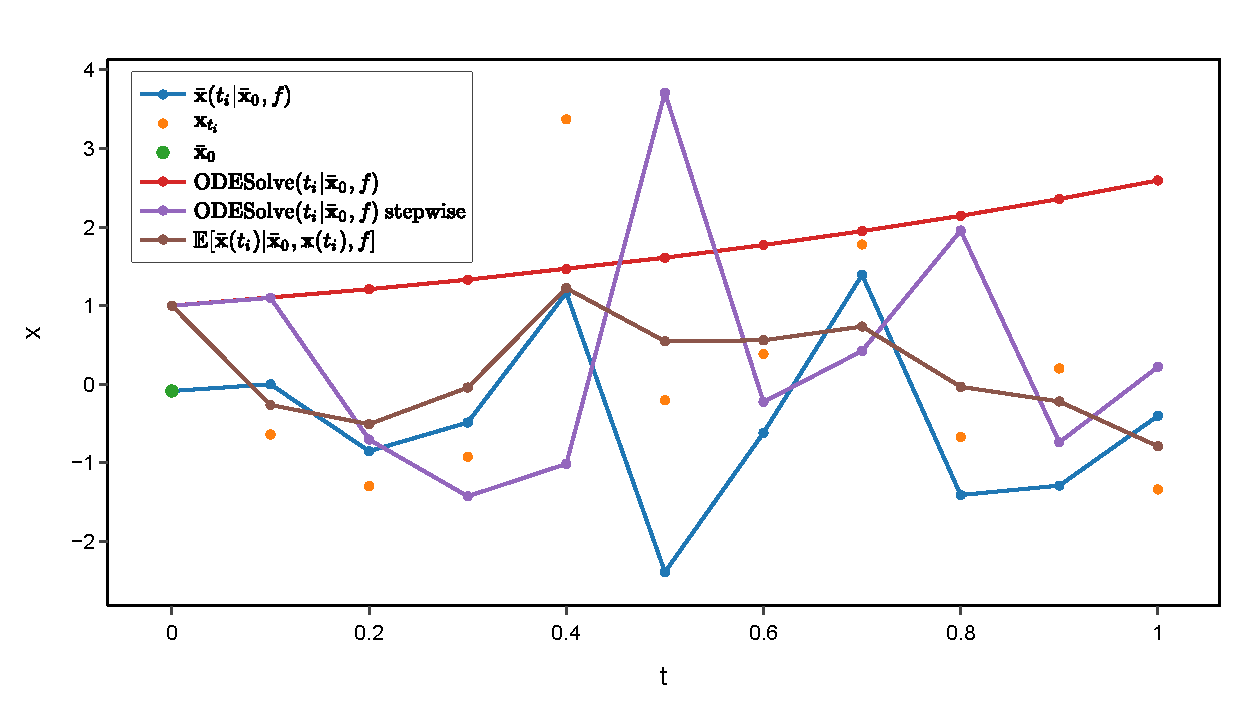
\includegraphics[width=0.38\textwidth, keepaspectratio]{img/sde_cls_compare}
			\caption*{\footnotesize СДУ $dx = x\,dt + dW(t)$: метод Эйлера расходится, UKF учитывает $dW$ и точнее всех с вероятностью $0.97$ по оценке Монте-Карло}
		\end{figure}

	\end{frame}

	\begin{frame}{Теоретическое обоснование аппроксимации полей методом NeuralODE через GMM}

		Из модели наблюдений следует моментное условие
		\begin{equation*}
			\mathbb{E} \left[ \bx_{t_i} -  \text{ODESolve}(t_i \,|\, \bbx_0, f) \right]  = 0, \quad i \in 1 \ldots n.
		\end{equation*}
		Обобщённый метод моментов (GMM): ищем поле в параметрическом классе $\mathcal{S}_{\Theta}$, минимизируя по коротким батчам временных рядов $B_j$ (NODE, градиентная оптимизация):
		\begin{equation*}
			\sum\limits_{j=1}^N \sum\limits_{\bbx_0, \bx_{t_i} \in B_j} \big\lVert  \bx_{t_i} -  \text{ODESolve}(t_i \,|\, \bbx_0, f) \big\rVert_2^2 \to \underset{f \in \mathcal{S}_{\Theta}}{\min}.
		\end{equation*}

		\begin{block}{Гарантия состоятельности}
			При выполнении технических условиях GMM на $\Theta$ имеем
			\begin{equation*}
				f_{\hat{\Theta}} \xrightarrow{\ \mathbb{P}\ } f, \quad n \to \infty.
			\end{equation*}
		\end{block}

		Короткие батчи ограничивают накопление ошибки ODESolve. Для СДУ-динамики существуют аналоги NeuralODE.

	\end{frame}
	
	\begin{frame}{Постановка вычислительных экспериментов}
	
	\textbf{Цели}
	
	\begin{enumerate}
		\item Эмпирически оценить качество классификации метрического классификатора на синтетических и реальных данных.
		\item Сравнить с другими методами, использующие динамические системы: RNN и $k$-NN классификатор с dynamic time warping (DTW) метрикой.
	\end{enumerate}
	
	\textbf{Датасеты}
	
	\begin{enumerate}
		\item Сэмплирование из трёх различных линейных ОДУ вида $f(\bbx) = A \bbx$
		\item MotionSense --- показания акселерометра и гироскопа для разных типов движений человека
	\end{enumerate}
	
	Во всех экспериментах для вычисления $\mathbb{E}[\bbx(t_i) \,|\, \bbx_0, \bx(t_i), f]$ использовался UKF фильтр + RTS сглаживание.
	\end{frame}

	\begin{frame}{Линейные ОДУ с общим типом динамики}

		Три системы с общим спектром $\Lambda$ и разными базисами $U$ (затухающие колебания + экспоненциальное затухание):
		\begin{equation*}
			f(\bbx) = U  \begin{pmatrix}
				-\gamma_1 & w & 0 \\
				-w & -\gamma_1 & 0 \\
				0 & 0 & -\gamma_2
			\end{pmatrix} U^{\text{T}} \bbx.
		\end{equation*}
		Длина ряда $n = 100$, уровень шума $\sigma = 2$.

		\begin{columns}[T]
			\begin{column}{0.52\textwidth}
				\centering
				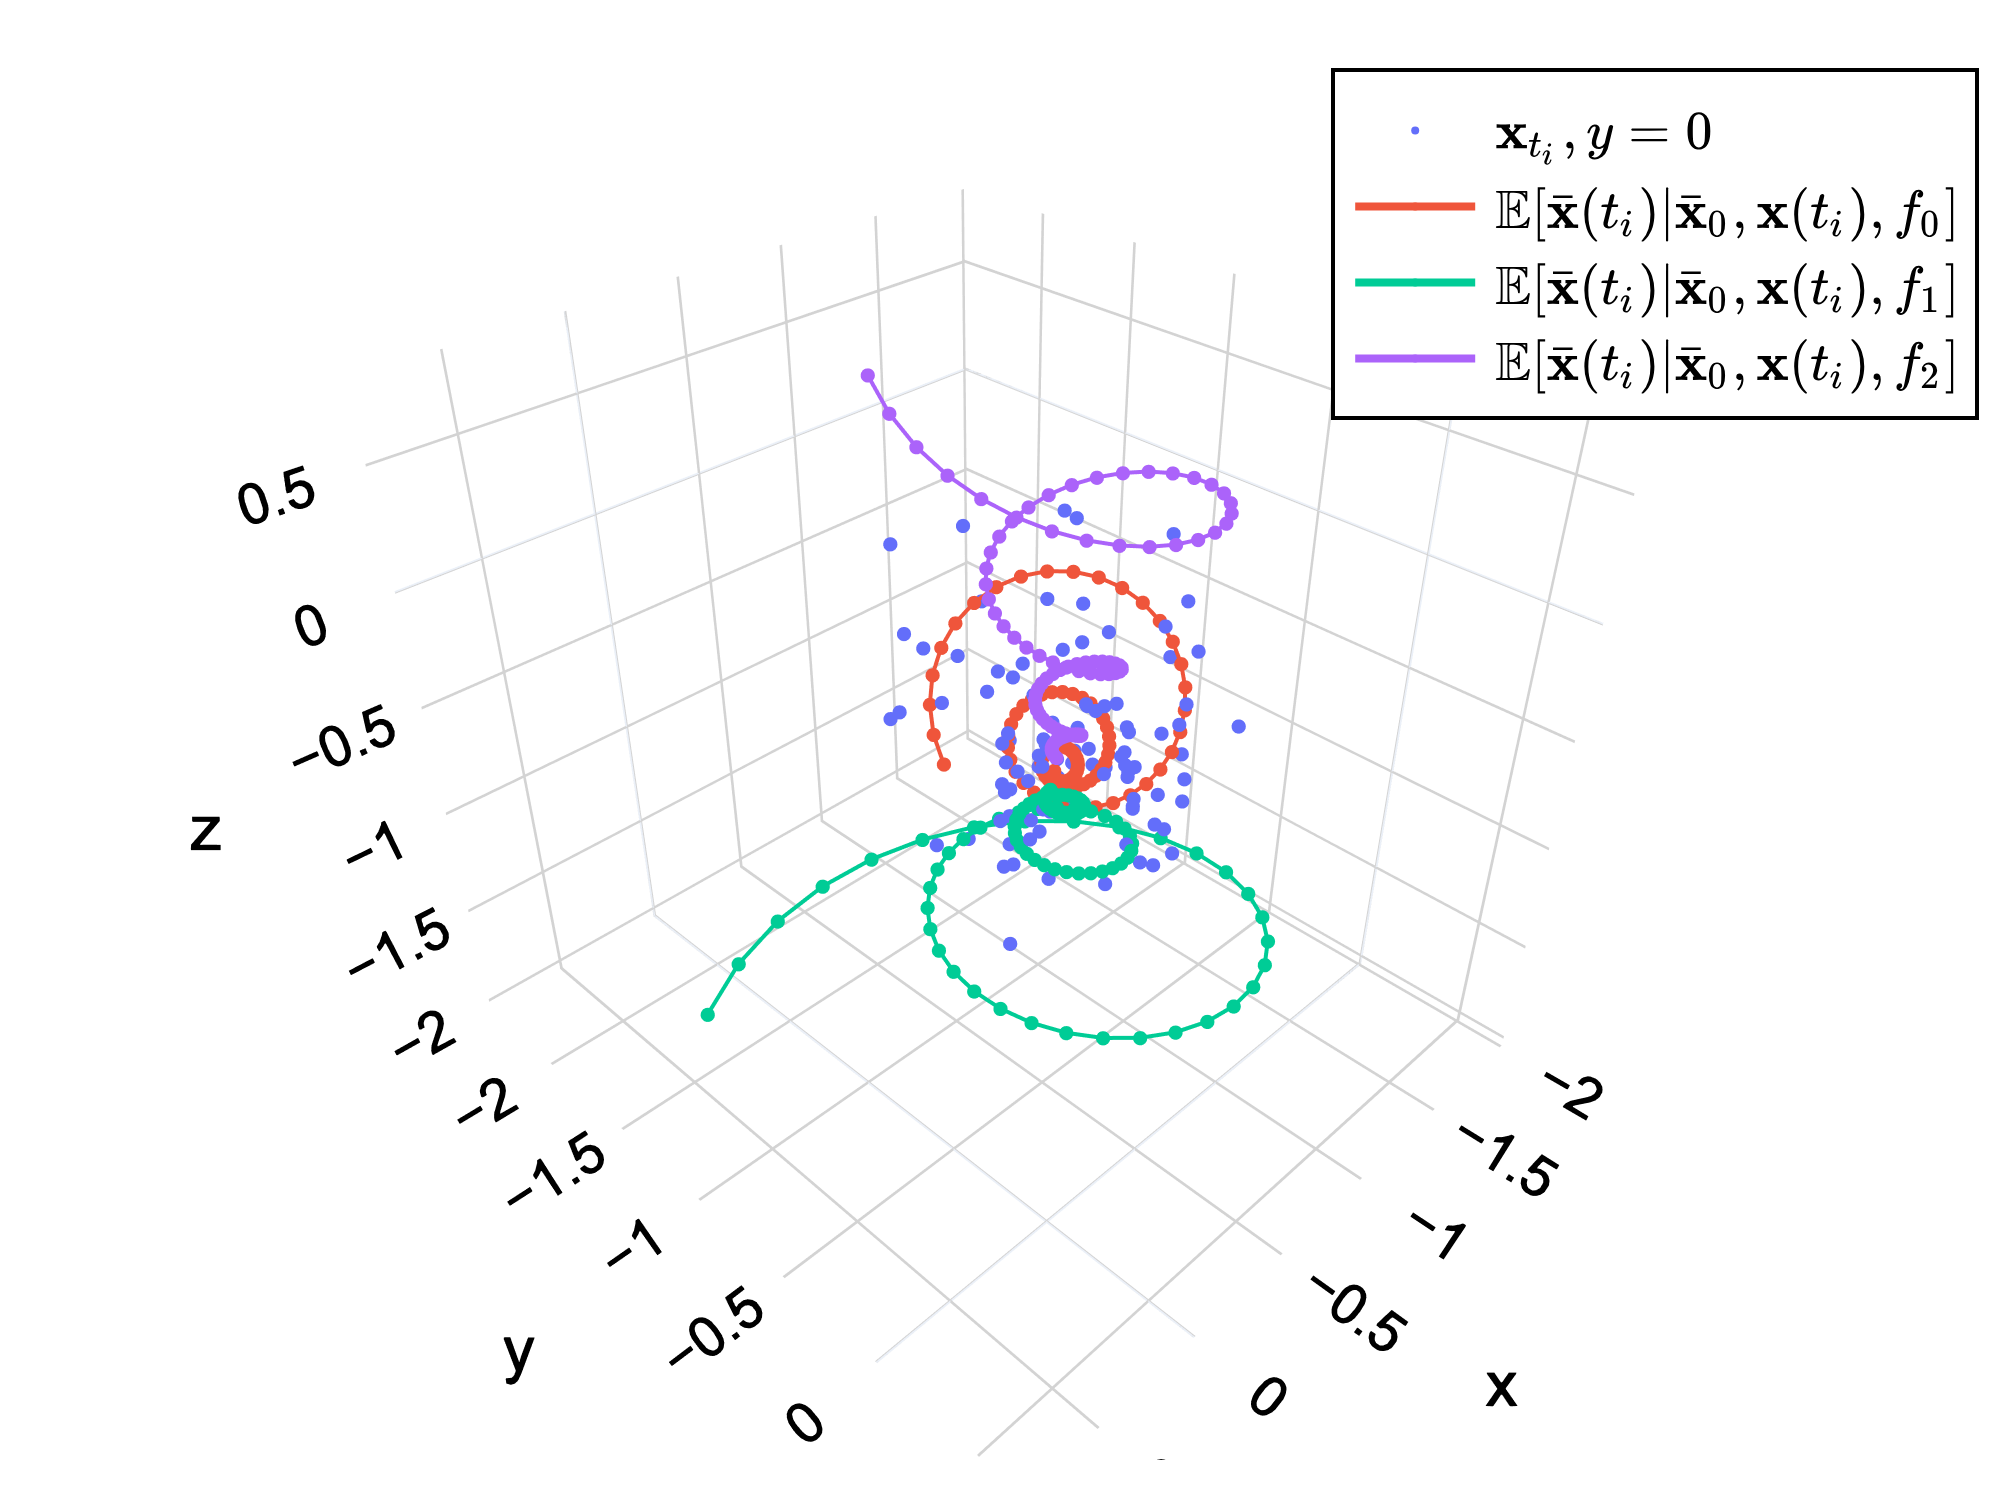
\includegraphics[width=\linewidth, keepaspectratio]{img/linear_system_0}
			\end{column}
			\begin{column}{0.44\textwidth}
				\centering
				\vspace{1em}
				\begin{tabular}{lc}
					\toprule
					Метод & Accuracy \\
					\midrule
					$k$-NN + DTW & 0.67 \\
					LSTM & 0.27 \\
					UKF+RTS & \textbf{0.86} \\
					\bottomrule
				\end{tabular}

				\vspace{1em}
				\footnotesize LSTM не различает системы из-за сильного шума и общего $\Lambda$; DTW субоптимален по метрике и использованию $f_j$.
			\end{column}
		\end{columns}

	\end{frame}

	\begin{frame}{MotionSense: движение человека как механическая система}

		\textbf{Постановка}: IMU-сигналы $50$ Гц (угловая скорость + ускорение, $d = 6$), 6 субъектов, 6 активностей-классов: ходьба, бег, лестница вверх/вниз, статичное положение стоя и сидя. Поля $f_j$ неизвестны --- учим из данных.

		\vspace{0.4em}
		\textbf{Мотивация ОДУ}: человек --- система твёрдых тел, движение описывается уравнениями Лагранжа вида (\ref{eq:lat_dyn}). Активные движения --- предельные циклы, статичные движения --- устойчивые равновесия. Поэтому ищем поле в виде $f(\bbx) = A \bbx + \text{NN}(\bbx)$, где $A \bbx$ задаёт тип динамики, $\text{NN}$ учитывает нелинейные детали движений.

		\vspace{0.4em}
		\textbf{Гипотеза индивидуальности}: движения человека имеют множество особенностей $\Rightarrow$ каждый субъект имеет уникальное поле $f_{\text{subj}_j}$ для каждого движения. Нулевая гипотеза: все $f_{\text{subj}_j}$ одинаковы $\Rightarrow$ классификатор субъектов:
		\begin{equation*}
			\delta \big( \bx(t_i) \big) = \underset{j \in 1 \ldots \text{num subjects}}{\arg\min} \ \rho_n\big( \bx(t_i), \mathbb{E}[\bbx(t_i) \,|\, \bbx_0, \bx(t_i), f_{\text{subj}_j}] \big)
		\end{equation*}
		случен, т.е. его accuracy $ = 0.5$.

	\end{frame}

	\begin{frame}{Сглаженные траектории разделяют активности}

		\begin{figure}[h]
			\centering
			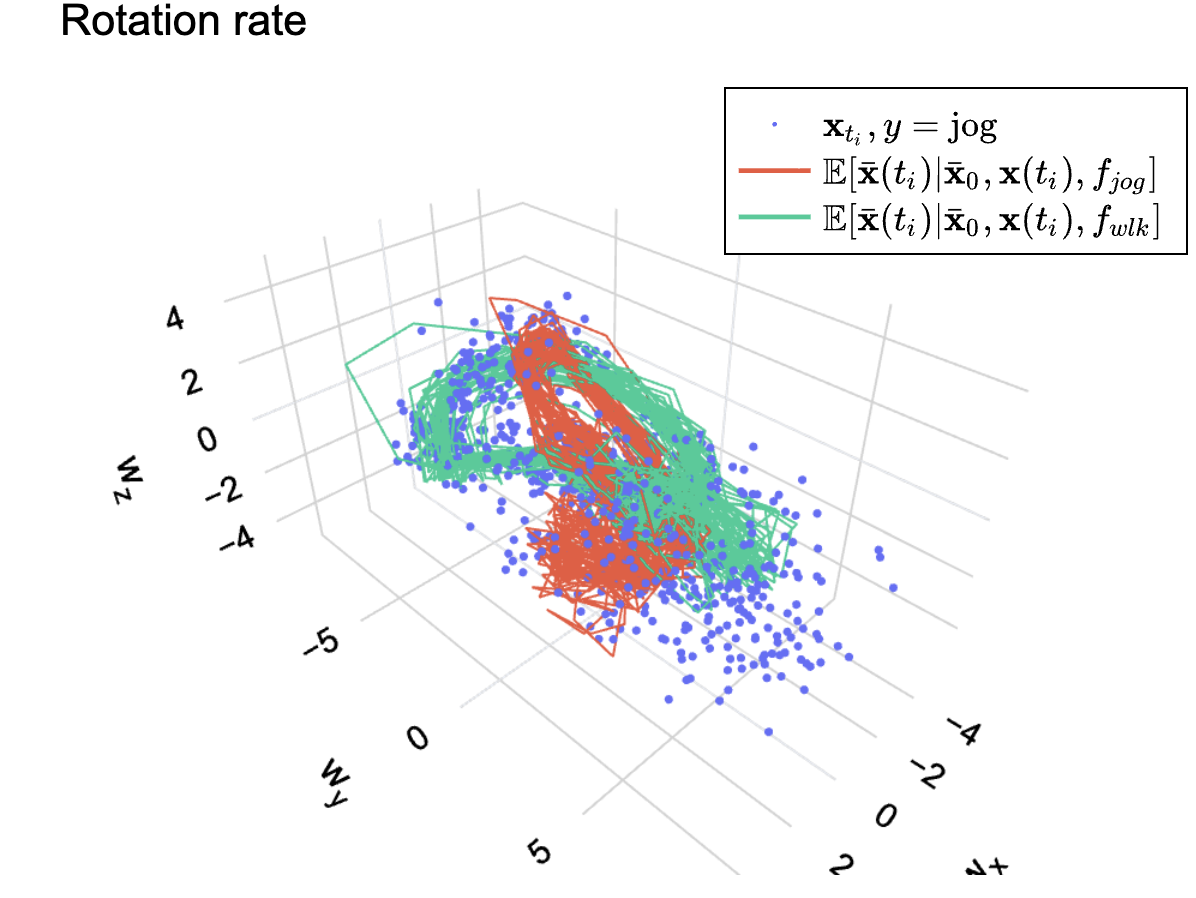
\includegraphics[width=0.35\textwidth, keepaspectratio]{img/rotrate_jog_smooth}
			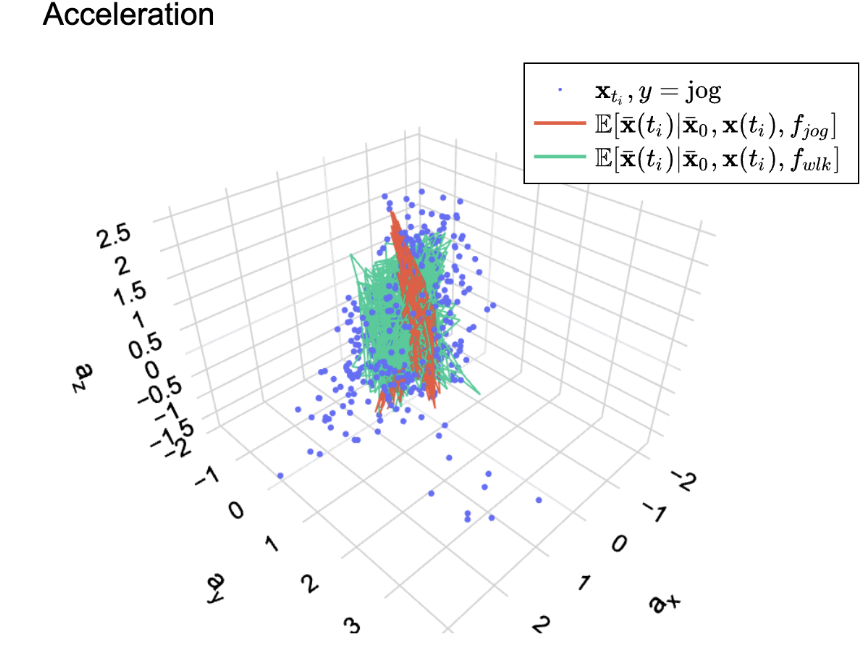
\includegraphics[width=0.35\textwidth, keepaspectratio]{img/accel_jog_smooth}

			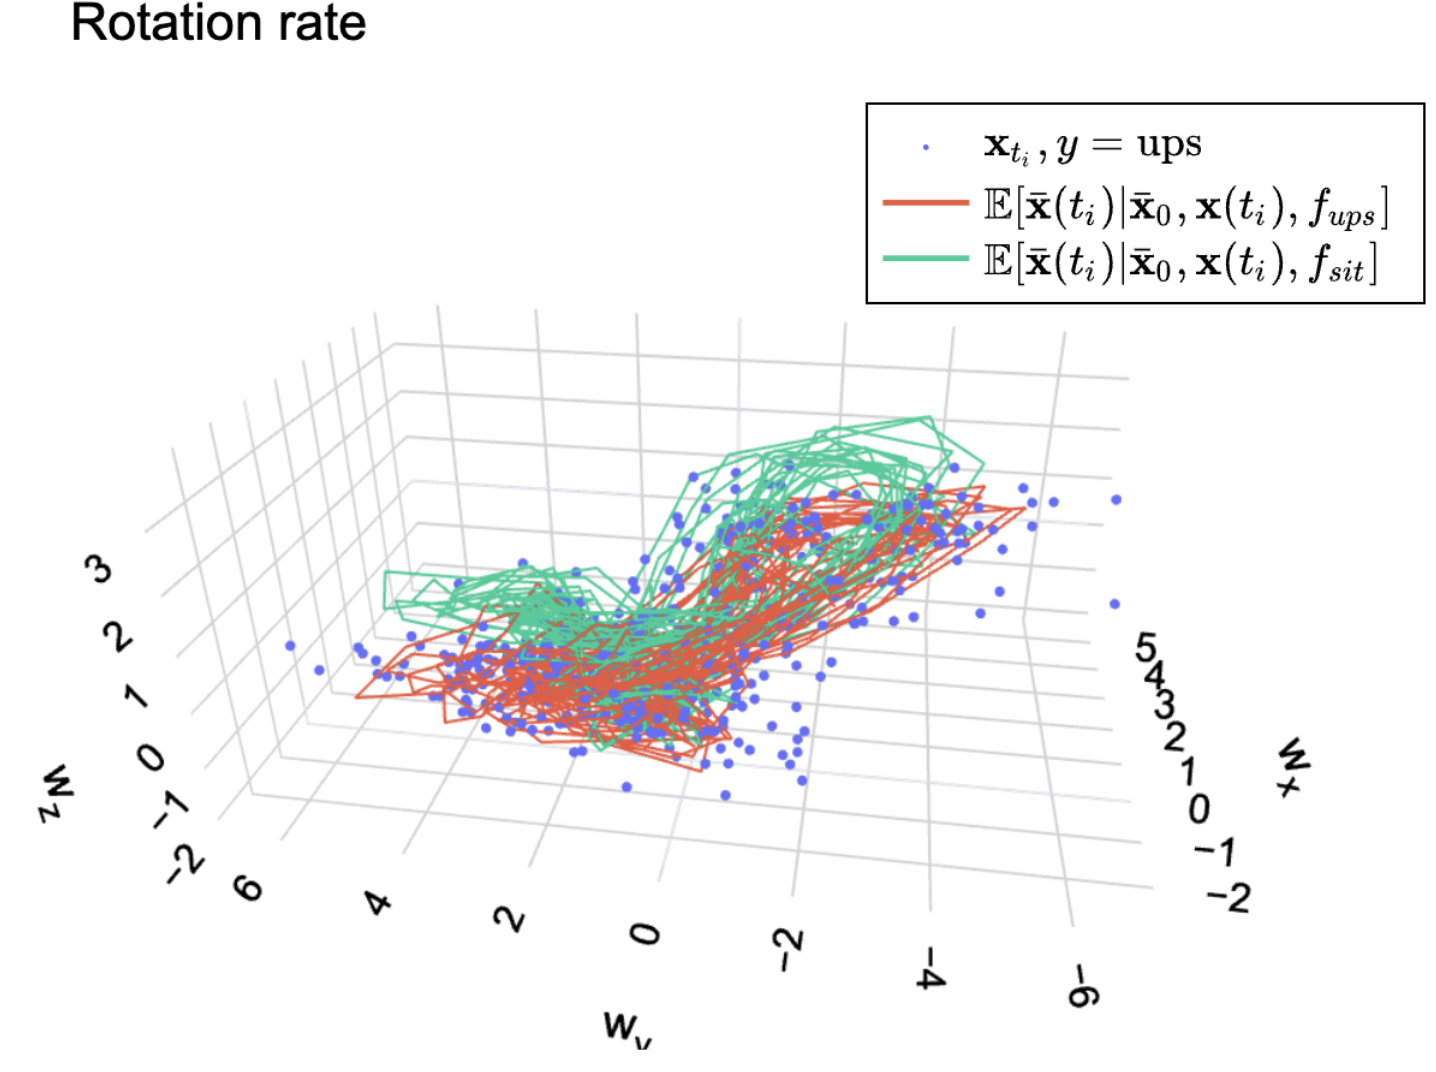
\includegraphics[width=0.35\textwidth, keepaspectratio]{img/rotrate_ups_smooth}
			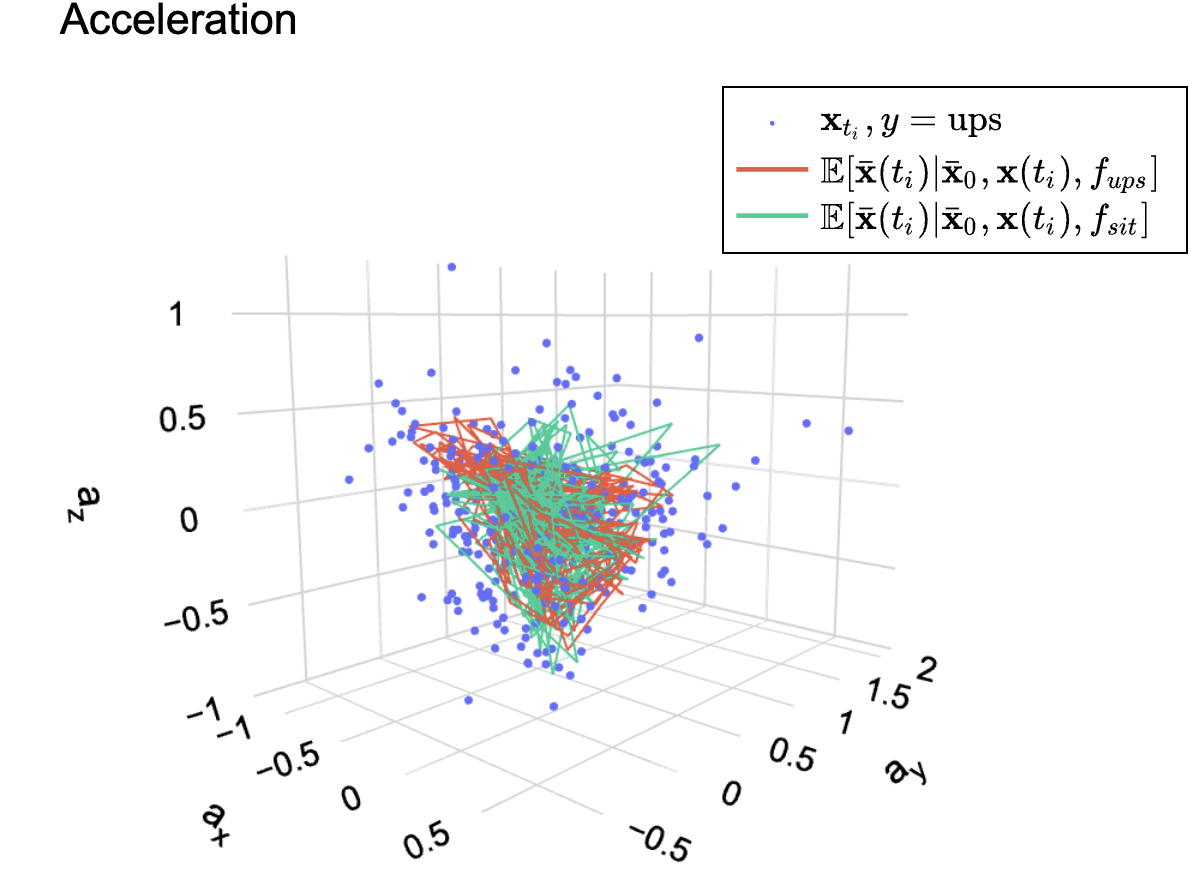
\includegraphics[width=0.35\textwidth, keepaspectratio]{img/accel_ups_smooth}
			\caption*{\footnotesize Сверху: бег, сглаживание полями $f_{\text{jog}}$ и $f_{\text{wlk}}$. Снизу: лестница вверх, поля $f_{\text{ups}}$ и $f_{\text{sit}}$. «Своё» поле следует за рядом точнее чужого.}
		\end{figure}

	\end{frame}

	\begin{frame}{Валидация ОДУ-модели}

		\begin{columns}[T]
			\begin{column}{0.48\textwidth}
				\centering
				\textbf{Классификация активностей}

				\vspace{0.5em}
				\footnotesize
				\begin{tabular}{lc}
					\toprule
					Активность & Accuracy \\
					\midrule
					jog & 0.84 \\
					walk & 0.84 \\
					upstairs & 0.72 \\
					downstairs & 0.70 \\
					stand & 0.75 \\
					sit & 0.74 \\
					\textbf{все} & \textbf{0.765} \\
					\bottomrule
				\end{tabular}
			\end{column}
			\begin{column}{0.48\textwidth}
				\centering
				\textbf{Тест индивидуальности}

				\vspace{0.5em}
				\footnotesize
				\begin{tabular}{lcc}
					\toprule
					Активность & p-value & Accuracy \\
					\midrule
					jog & \textbf{0.03} & 0.84 \\
					walk & \textbf{0.01} & 1.00 \\
					upstairs & 0.35 & 0.68 \\
					downstairs & 0.34 & 0.71 \\
					stand & 0.41 & 0.65 \\
					sit & 0.89 & 0.34 \\
					\bottomrule
				\end{tabular}
			\end{column}
		\end{columns}

		\vspace{1em}
		Общая точность $0.765$ в целом подтверждает ОДУ-модель. $H_0$ отвергнута для бега и ходьбы --- наиболее сложных и динамичных движений. Для статичных поз индивидуальности не обнаружена, как и в ходьбе по лестнице.

	\end{frame}

	\begin{frame}{Выносится на защиту}

		\begin{enumerate}
			\item Метод классификации временных рядов в модели динамических систем ОДУ/СДУ с учётом случайного шума.
			\item Теорема об асимптотической оптимальности классификатора при известных полях и начальной точке; обоснование перехода к задаче сглаживания при нарушении этих условий.
			\item Процедура состоятельного обучения векторных полей по данным (NODE + GMM).
			\item Эмпирическая валидация на синтетических линейных системах и на данных MotionSense (accuracy $0.765$). Формализция гипотезы индивидуальности движений и её проверка.
		\end{enumerate}

	\end{frame}

\end{document}
